% L’utilisateur connecté au bureau virtuel pourra lancer un widget au travers d’un lanceur. Celui-ci s’apparentera au dock du système 
% d’exploitation Mac. Cela ne sera possible que si le nombre de widgets ouverts n’a pas atteint sa valeur maximale.

% L’utilisateur pourra ouvrir une fenêtre de type calculatrice et saisir une addition ou une soustraction. Le résultat apparaîtra sur 
% l’écran de tous les utilisateurs.

% Un utilisateur pourra aussi lancer le widget bloc-notes, permettant de saisir du texte et ainsi de l’afficher auprès des autres machines clientes.

% Un widget « Photos » pourra être utilisé afin de faire défiler quelques images pré-chargées sur le serveur.

% L’utilisateur connecté au bureau virtuel pourra quitter l’application via un bouton disponible dans le dock de lancement.

\section{Scénario d'utilisation 1}
\begin{itemize}
	\item Nom : Se connecter au serveur;
	\item Description : L'utilisateur accède au bureau virtuel via le programme correspondant;
	\item Acteurs : Utilisateur du bureau virtuel.
\end{itemize}

\paragraph{Séquence d'événements}
\begin{itemize}
	\item L'utilisateur lance le programme "bureau virtuel" sur son ordinateur personnel;
	\item Le serveur vérifie si le nombre d'utilisateurs ne dépasse pas la limite;
	\item L'utilisateur accède au bureau virtuel.
\end{itemize}

\paragraph{Exceptions}
\begin{itemize}
	\item L'utilisateur lance le programme;
	\item Le nombre d'utilisateur dépasse la limite;
	\item L'utilisateur est invité à réessayer de se connecter plus tard, lorsqu'un utilisateur se sera déconnecté.
\end{itemize}

% ------------------------------------

\section{Scénario d'utilisation 2}
\begin{itemize}
	\item Nom : Ouvrir une fenêtre;
	\item Description : L'utilisateur ouvre une des fenêtres disponibles sur le bureau;
	\item Acteurs : Utilisateur du bureau virtuel;
	\item Préalable : L'utilisateur est connecté au serveur.
\end{itemize}

\paragraph{Séquence d'événements}
\begin{itemize}
	\item L'utilisateur clique sur l'une des icônes disponibles représentant un widget;
	\item Le serveur vérifie que le nombre de fenêtres est inférieur à 6;
	\item Si le nombre de fenêtres ouvertes est inférieur à 6, le widget s'ouvre.
\end{itemize}

\paragraph{Exceptions}
\begin{itemize}
	\item L'utilisateur clique sur un lanceur;
	\item Le nombre de widgets ouverts est de 6 ou plus;
	\item Un message d'erreur apparaît invitant l'utilisateur à fermer une fenêtre pour en ouvrir une autre.
\end{itemize}

% ------------------------------------
{\color{red}
\section{Scénario d'utilisation 3}
\begin{itemize}
	\item Nom : Saisir une opération;
	\item Description : L'utilisateur saisit une opération sur le widget Calculatrice;
	\item Acteurs : Utilisateur du bureau virtuel;
	\item Préalable : L'utilisateur est connecté au serveur, un widget Calculatrice est ouvert.
\end{itemize}

\paragraph{Séquence d'événements}
\begin{itemize}
	\item L'utilisateur clique sur le bouton représentant le premier opérande;
	\item L'utilisateur clique sur le bouton représentant l'opérateur;
	\item L'utilisateur clique sur le bouton représentant le second opérande;
	\item L'utilisateur clique sur le symbole "=";
	\item Le résultat est affiché.
\end{itemize}
}

% ------------------------------------

\section{Scénario d'utilisation 4}
\begin{itemize}
	\item Nom : Regarder des photos;
	\item Description : L'utilisateur utilise le widget Galerie;
	\item Acteurs : Utilisateur du bureau virtuel;
	\item Préalable : L'utilisateur est connecté au serveur, un widget Galerie est ouvert.
\end{itemize}

\paragraph{Séquence d'événements}
\begin{itemize}
	\item L'utilisateur clique sur le bouton d'afficher l'image suivante;
	\item L'utilisateur clique sur le bouton d'afficher l'image précédente.
\end{itemize}


% ------------------------------------

\section{Scénario d'utilisation 5}
\begin{itemize}
	\item Nom : Quitter le bureau virtuel;
	\item Description : L'utilisateur se déconnecte du serveur;
	\item Acteurs : Utilisateur du bureau virtuel;
	\item Préalable : L'utilisateur est connecté  au serveur.
\end{itemize}

\paragraph{Séquence d'événements}
\begin{itemize}
	\item L'utilisateur clique sur le bouton "Déconnexion";
	\item Une fenêtre de confirmation s'ouvre demandant à l'utilisateur de cliquer sur "confirmer" ou "annuler";
	\item L'utilisateur clique sur "confirmer";
	\item L'utilisateur est déconnecté du serveur.
\end{itemize}

{\color{red}
Ce diagramme résume les différents cas d'utilisation définis dans le dossier de spécifications externes.

\begin{figure}[H]
	\centering
	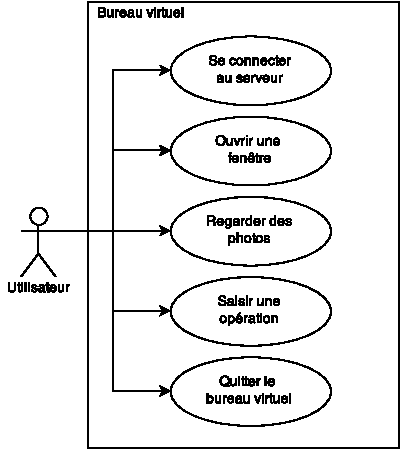
\includegraphics[scale=0.8]{diagrammes/DCU.pdf}
	\caption{Diagramme des cas d'utilisation}
\end{figure}
}